\documentclass[letter, 10pts]{article}
\usepackage[monocolor]{../math232/ahsansabit}
\usepackage[]{float}
\usepackage{tikz}
\usepackage{tikz-3dplot}
\usepackage[outline]{contour} % glow around text
\usepackage{xcolor}
\usepackage{pdfpages}
\usepackage{physics}
\usepackage{multicol}
\title{Quantum Mechanics : : Homework 09}
\author{Ahmed Saad Sabit, Rice University}
\date{\today}
\newcommand{\hb}{\hbar}
\newcommand{\U}{\uparrow}
\newcommand{\D}{\downarrow}
\usepackage[]{braket}
\begin{document}
\maketitle

\section*{Problem 01}
\begin{minipage}{0.5\textwidth}
\begin{align*}
	\bra{x}	\hat{P}^2 \ket{\psi} &= 
	\bra{x} \hat{P}^2 \ket{x'} \braket{x'|\psi} \\
	&=  
	\bra{x} \hat{P}^2 \ket{x'} \psi(x') \\
	&= (-i \hb)^2 \frac{\mathrm{d} ^2}{\mathrm{d} x^2} \psi(x) \\
	&= - \hb^2 \frac{\mathrm{d} ^2}{\mathrm{d} x^2} \psi(x) 
\end{align*}
\end{minipage}\hfill\begin{minipage}{0.5\textwidth}
\begin{align*}
	\hat{H} \ket{\psi} = E \ket{\psi} \implies \hat{H} \ket{\psi} &= 0 \\ 
	\left(\frac{\hat{P}^2}{2m} + \frac{V_0}{a} \hat{X}\right) \ket{\psi} &= 0\\
\left(\frac{\hat{P}^2}{2m} + \frac{V_0}{a} \hat{X}\right) \ket{x} \braket{x|\psi} &= 0\\
\left(\frac{\hat{P}^2}{2m} \ket{x}+ \frac{V_0}{a} x \right) \psi_0(x) &= 0\\
\left(-\frac{\hb ^2}{2m} \frac{\mathrm{d} ^2}{\mathrm{d} x^2}  + \frac{V_0}{a} x \right) \psi_0(x) &= 0\\ \implies
-\frac{\hb ^2}{2m} \frac{\mathrm{d} ^2 \psi_0(x)}{\mathrm{d} x^2}  + \frac{V_0}{a} x \psi_0(x) &= 0\\
\end{align*}
\end{minipage} 


\subsection*{(a)} 
The zero energy eigenstate is given by 
\[
\psi_0(x) =
\frac{c}{\sqrt{2 \pi \hb} }
\int_{-\infty}^{\infty} 
\mathrm{d} p\, 
e^{ipx / \hb}
\exp 
\left(
i \frac{a}{\hb V_0} \left(\frac{p^3}{6m}\right)
\right)
\] 
Complex Conjugate
\begin{align*}
	\psi_0(x)^{*} &=
\frac{c^{*}}{\sqrt{2 \pi \hb} }
\int_{-\infty}^{\infty} 
\mathrm{d} p\, 
e^{-ipx / \hb}
\exp 
\left(
- i \frac{a}{\hb V_0} \left(\frac{p^3}{6m}\right)
\right) 
\\
	&=
\frac{c^{*}}{\sqrt{2 \pi \hb} }
\int_{-\infty}^{\infty} 
\mathrm{d} p\, 
e^{i(-p)x / \hb}
\exp 
\left(
 i \frac{a}{\hb V_0} \left(\frac{(-p)^3}{6m}\right)
\right) \\
	&= - 
\frac{c^{*}}{\sqrt{2 \pi \hb} }
\int_{\infty}^{-\infty} 
\mathrm{d} u\, 
e^{i u x / \hb}
\exp 
\left(
 i \frac{a}{\hb V_0} \left(\frac{u^3}{6m}\right)
\right) \tag{$ - p : = u$}
\\ 	&= 
\frac{c^{*}}{\sqrt{2 \pi \hb} }
\int_{-\infty}^{\infty} 
\mathrm{d} u\, 
e^{i u x / \hb}
\exp 
\left(
 i \frac{a}{\hb V_0} \left(\frac{u^3}{6m}\right)
\right) 
\end{align*} 
Taking the complex conjugate we can see that the integral is the same with a new dummy variable $u$ from $p$. For the integral, the original and it's complex conjugate being the same means the integral itself is purely real. 

For the normalization constant $c$, when we compute $\psi^{*} \nabla \psi$, then we get a factor $c^{*} c = |c|^2$ which is purely real. Hence $\psi ^{*} \nabla \psi$ has practically no imaginary part meaning $J(x) = 0$. 

$\psi$ is a standing wave without time dependence so they are constant in time.





\subsection*{(b)} 
\begin{align*}
	\frac{\mathrm{d} \braket{X }}{\mathrm{d} t} &= \frac{\braket{ P}}{m} \\
	\frac{\mathrm{d} \braket{P }}{\mathrm{d} t} &= - \frac{i}{\hb} \braket{[\hat{H} , \hat{P}]} 
= i \hb \frac{V_0}{ a} \left(- \frac{i}{\hb}\right) = - \frac{V_0}{a}
	\\
	\implies \braket{ P} &= p_0 - \frac{V_0}{a}t
	\\ \implies
	\braket{ X} &=  \int_{}^{} \mathrm{d} t \, \braket{ P} \frac{1}{m} = x_0 + \frac{p_0}{m}t  - \frac{V_0}{2 a m } t^2  \\
\end{align*}
\begin{comment} 
\begin{align*}
	\braket{\hat{X} } &= \bra{\psi(0)} \hat{X} \ket{\psi(0)} = x_0	
			  & \braket{ \hat{P}} &= \bra{\psi(0)} \hat{P} \ket{\psi(0)}  = p_0
\end{align*}
\begin{align*}
\ket{\psi(t)} &= \hat{U}(t) \ket{\psi_0} \\
&= e^{- i \hat{H} t / \hb} \ket{\psi_0} \\
\bra{\psi(t)} &= \bra{\psi_0} e^{i \hat{H} t / \hb}
\end{align*}

\begin{align*}
	\braket{ \hat{X}} &= \bra{\psi(t)} \hat{X} \ket{\psi(t)} \\
	&= \int_{-\infty}^{\infty} \int_{-\infty}^{\infty}  \mathrm{d} x' \, \mathrm{d} x \,  
\braket{\psi(t) | x'} \bra{x'} \hat{X} \ket{x} \braket{x | \psi(t)} 
\\
	&= \int_{-\infty}^{\infty} \int_{-\infty}^{\infty}  \mathrm{d} x' \, \mathrm{d} x \,  
\braket{\psi(0)| e^{i \hat{H} t / \hb} | x'} \bra{x'} \hat{X} \ket{x} \braket{x | e^{- i \hat{H} t / \hb} | \psi(0)}
	\\
	&= \int_{-\infty}^{\infty} \int_{-\infty}^{\infty}  \mathrm{d} x' \, \mathrm{d} x \,  
	\left[\left(
			e^{i E_n t / \hb}
	\right)
\braket{\psi(0)| x'} \right]
x \, \delta(x  - x' )
	\left[\left(
			e^{- i E_n t / \hb}
	\right)
\braket{x| \psi(0)} \right]
	\\
	&= \int_{-\infty}^{\infty}  \mathrm{d} x \,  
	\psi^{*}(x)
\, x \, 
\psi(x)
	\\
\end{align*}
\end{comment}




\section*{Problem 02} 
If $k = \sqrt{2 \mu E / \hb ^2} $ then the wave function is given by 
\[
	\psi_{E,m}(r, \phi) = 
	A e ^{i m \phi} J_m (kr)
\] 
The current density is given by 
\[
\vec{J} = 
\frac{\hb}{\mu} \text{Im} \left(\psi ^{*} \vec{\nabla} \psi\right)
\]
Firstly computing the gradient 
\begin{align*}
	\vec{\nabla} \psi &= 
\vec{n}_r \frac{\partial}{\partial r} 
	\left(A e ^{i m \phi} J_m (kr)\right) + 
	+ 
	\vec{n}_\phi \frac{1}{r} 
	\frac{\partial }{\partial \phi}
	\left(A e ^{i m \phi} J_m (kr)\right)  \\ 
	&= 
\vec{n}_r A e^{i m \phi} 
\frac{\partial J_m(kr)}{\partial r} 
+ 
\vec{n}_\phi \frac{A e^{im \phi}J_m(kr)}{r}(i m)
	\\
\end{align*}
Computing the complex conjugate now 
\[
\psi^{*} = A^{*} e^{- i m \phi} J_m (kr)
\]
\begin{align*}
	\psi^{*} \vec{\nabla} \psi &= \vec{n}_r A A^{*} J_m(kr) 
\frac{\partial J_m(kr)}{\partial r}
+ 
\vec{n}_\phi \frac{A A^{*} J_m^2(kr)}{r}(i m)
				\\ &=
	\underbrace{
\vec{n}_r 
\frac{|A|^2}{2} \frac{\partial ^2}{\partial r ^2} [J^2_m(kr)]}_{\text{purely real}} + \vec{n}_\phi \left(i\right)
	\frac{m|\psi_{E,m}|^2} {r} \\ 
	\text{Im} \left(\psi ^{*} \vec{\nabla} \psi \right) &= \vec{n}_\phi \frac{m}{r} |\psi_{E,m} | ^2
\end{align*}
From this it shows, 
\[
	\vec{J} (r,\phi) = \vec{n}_\phi \frac{m \hb }{ \mu r} |\psi_{E,m}(r)|^2  = 
	\vec{n}_\phi \frac{m \hb }{ \mu r} \rho(r)
\]
Note that $\psi(r,\phi)$ becomes only a function of $r$ when it's magnitude is taken because of the $e^{i m \phi}$ term vanishing while taking the complex conjugate.

\textbf{Interpretation:}

Classical particle angular momentum when it rotates along $z$ axis 
\[
L _z = m r^2 \omega  = m v r
\] 
\[
v = \frac{L_z}{\mu r}
\] 
Quantum Mechanically we can treat $L_z = \hb m$ so we have got a somewhat analogous classical particle 
\[
v = \frac{m \hb}{\mu r}
\] 

\section*{Problem 03}
\subsection*{(a)} 
\begin{align*}
	\psi(x,t) &= \braket{x | \psi(t)}  \\
	&= \braket{x | \hat{U}(t) | \psi(0)} \\
	&= \braket{x | \hat{U}(t) \hat{I} | \psi(0)} \\
	&= \int_{-\infty}^{\infty} \mathrm{d} x' \, 
	\braket{x | \hat{U}(t) | x'} \braket{x' | \psi(0)}\\
	&= \int_{-\infty}^{\infty} \mathrm{d} x' \, 
	U(x,x'; t) \psi_0 (x') \\
	&= \int_{-\infty}^{\infty}   
	\mathrm{d} x' \, 
	\left(\frac{1}{2 \pi i \lambda(t) \Delta_0 ^2}\right) 
	^{1 / 2} 
	\exp
	\left(
\frac{i(x-x')^2}{2 \lambda(t) \Delta_0^2}
	\right)
\psi_0(x')
	\\
	&= 
	\left(\frac{1}{2 \pi i \lambda(t) \Delta_0 ^2}\right) 
	^{1 / 2} 
	\int_{-\infty}^{\infty}   
	\mathrm{d} x' \, 
	\exp
	\left(
\frac{i(x-x')^2}{2 \lambda(t) \Delta_0^2}
	\right)
\psi_0(x')
	\\
	&= 
	\left(\frac{1}{2 \pi i \lambda(t) \Delta_0 ^2}\right) 
	^{1 / 2} 
	\int_{-\infty}^{\infty}   
	\mathrm{d} x' \, 
	\exp
	\left(
\frac{i(x-x')^2}{2 \lambda(t) \Delta_0^2}
	\right)\left[
	\left(\frac{1}{\pi \Delta_0^2}\right)^{1 / 4} 
	\exp\left(
- \frac{(x'-x_0)^2}{2 \Delta_0^2}
\right)\right]
	\\
	&= 
	\left(\frac{1}{\pi \Delta_0^2}\right)^{1 / 4} 
	\left(\frac{1}{2 \pi i \lambda(t) \Delta_0 ^2}\right) 
	^{1 / 2} 
	\int_{-\infty}^{\infty}   
	\mathrm{d} x' \, 
	\exp
	\left(
\frac{i(x-x')^2}{2 \lambda(t) \Delta_0^2}
	\right)\left[
	\exp\left(
- \frac{(x'-x_0)^2}{2 \Delta_0^2}
\right)\right]
	\\
	&= 
	\left(\frac{1}{\pi \Delta_0^2}\right)^{1 / 4} 
	\left(\frac{1}{2 \pi i \lambda(t) \Delta_0 ^2}\right) 
	^{1 / 2} 
	\int_{-\infty}^{\infty}   
	\mathrm{d} x' \, 
	\exp
	\left(
\frac{i(x-x')^2}{2 \lambda(t) \Delta_0^2}
	\right)\left[
	\exp\left(
- \frac{(x'-x_0)^2}{2 \Delta_0^2}
\right)\right]
\\
	&= 
	\left(\frac{1}{\pi \Delta_0^2}\right)^{1 / 4} 
	\left(\frac{1}{2 \pi i \lambda(t) \Delta_0 ^2}\right) 
	^{1 / 2} 
	\int_{-\infty}^{\infty}   
	\mathrm{d} x' \, 
	\exp
	\left(
\frac{i(x-x')^2}{2 \lambda(t) \Delta_0^2}
	-
\frac{(x'-x_0)^2}{2 \Delta_0^2}
\right)
\\
	&= 
	\left(\frac{1}{\pi \Delta_0^2}\right)^{1 / 4} 
	\left(\frac{1}{2 \pi i \lambda(t) \Delta_0 ^2}\right) 
	^{1 / 2} 
	\int_{-\infty}^{\infty}   
	\mathrm{d} x' \, 
	\exp
	\left(
\frac{i
(x^2+x'^2- 2 x x')}{2 \lambda(t) \Delta_0^2}
	-
\frac{\lambda(t)(x'^2 + x_0^2 - 2 x_0 x')}{2 \lambda(t) \Delta_0^2}
\right) 
\\
	&= 
	\left(\frac{1}{\pi \Delta_0^2}\right)^{1 / 4} 
	\left(\frac{1}{2 \pi i \lambda(t) \Delta_0 ^2}\right) 
	^{1 / 2} 
	\int_{-\infty}^{\infty}   
	\mathrm{d} x' \, 
	\exp
	\left(
\frac{i
(x^2+x'^2- 2 x x')
- \lambda(t)(x'^2 + x_0^2 - 2 x_0 x')}{2 \lambda(t) \Delta_0^2}
\right) 
\\
	&= 
	\left(\frac{1}{\pi \Delta_0^2}\right)^{1 / 4} 
	\left(\frac{1}{2 \pi i \lambda(t) \Delta_0 ^2}\right) 
	^{1 / 2} 
	\int_{-\infty}^{\infty}   
	\mathrm{d} x' \, 
	\exp
	\left(
\frac{
i x^2+ i x'^2- 2 i  x x'
- \lambda(t) x'^2  - \lambda(t) x_0^2 + \lambda(t) 2 x_0 x'}{2 \lambda(t) \Delta_0^2}
\right) 
\\
	&= 
	\left(\frac{1}{\pi \Delta_0^2}\right)^{1 / 4} 
	\left(\frac{1}{2 \pi i \lambda(t) \Delta_0 ^2}\right) 
	^{1 / 2} 
	\int_{-\infty}^{\infty}   
	\mathrm{d} x' \, 
	\exp
	\left(
\frac{
i x^2- \lambda(t) x_0^2 + i x'^2  - \lambda(t) x'^2  - 2 i  x x'
+ \lambda(t) 2 x_0 x'}{2 \lambda(t) \Delta_0^2}
\right) 
\\
	&= 
	\left(\frac{1}{\pi \Delta_0^2}\right)^{1 / 4} 
	\left(\frac{1}{2 \pi i \lambda(t) \Delta_0 ^2}\right) 
	^{1 / 2} 
	\int_{-\infty}^{\infty}   
	\mathrm{d} x' \, 
	\exp
	\left(
\frac{
\left[ i x^2- \lambda(t) x_0^2
\right]
+ 
\left[
i   - \lambda(t)  \right] 
x'^2  + 
\left [- 2 i  x 
+ \lambda(t) 2 x_0 \right] 
x'}{2 \lambda(t) \Delta_0^2}
\right) 
\\
	&= 
	\left(\frac{1}{\pi \Delta_0^2}\right)^{1 / 4} 
	\left(\frac{1}{2 \pi i \lambda(t) \Delta_0 ^2}\right) 
	^{1 / 2} 
	\int_{-\infty}^{\infty}   
	\mathrm{d} x' \, 
	\exp
	\left(
	c
+ 
a x'^2
+  b
x'
\right) 
\impliedby
\begin{cases}
	a &= 
\left[
i   - \lambda(t)  \right] / 2 \lambda(t) \Delta_0^2  \\  
	b & =
\left [- 2 i  x 
+ \lambda(t) 2 x_0 \right]  / 2 \lambda(t) \Delta_0	^2 \\ 
c &=  
\left[ i x^2- \lambda(t) x_0^2
\right]  / 2 \lambda(t) \Delta_0^2
\end{cases}
\\
	&= 
	\left(\frac{1}{\pi \Delta_0^2}\right)^{1 / 4} 
	\left(\frac{1}{2 \pi i \lambda(t) \Delta_0 ^2}\right) 
	^{1 / 2} 
	\int_{-\infty}^{\infty}   
	\mathrm{d} x' \,  
	\exp(- b^2 / 4 a)
	\exp(c) \exp
	\left(
		a \left( x' + (b / 2a \right) )^2
\right) \\ 
\
\
\
&= 
	\left(\frac{1}{\pi \Delta_0^2}\right)^{1 / 4} 
	\left(\frac{1}{2 \pi i \lambda(t) \Delta_0 ^2}\right) 
	^{1 / 2}  
	\exp(- b^2 / 4 a)
	\exp(c) 
	\sqrt{\frac{\pi}{-a}}
	\\
&=
\text{paper and handheld basic algebra where I substitute the coefficients} \\ 
&=
\frac{1}{( 
	\sqrt{\pi } \Delta_0 [1 + i \lambda(t)]  
)^{\frac{1}{2}} }
\exp
\left(
- 
\frac{
	(x-x_0) ^2
}{2 \Delta_0^2 (1 + i \lambda(t ) ) }
\right)
\\
\end{align*}

\subsection*{(b)} 

\begin{align*}
	\psi_0(p) &= \int_{-\infty}^{\infty} \mathrm{d} x\,
	\psi_0 (x) e^{- i p x / \hb } \\ &=
\frac{1}{(\pi \Delta_0 ^2)^{1 / 2 }} 
\int_{-\infty}^{\infty} e^{- \frac{(x- x_0)^2}{2 \Delta_0^2} - i \frac{p x}{\hb}} 
\, \mathrm{d} x
\end{align*}
This above equation is almost like the gaussian we did in the class. On paper I do the following rough work to substitute the integral and we get, 
\[\boxed{
\psi_0(p) = 
\left(
\frac{2 \Delta_0^2}{ \pi }
\right)^{1 / 4} e^{ - i p x_0 / \hb } e^{ - \frac{\Delta_0 ^2 p^2}{2 \hb ^2}}
}\] 

\begin{align*}
	\braket{x | \psi} = 
	\psi(x,t) = 
	\left(\frac{2 \Delta_0^2 }{\pi }\right)^{1 / 4} 
	\frac{1}{\sqrt{2 \pi \hb}  } 
	\int_{-\infty}^{\infty} \mathrm{d} p \, 
	e^{i p x / \hb} 
	e^{- i p^2 t / 2 m \hb } 
	e^{- \Delta_0 ^2 p^2 / 2 \hb ^2}
	e^{ - i p x_0 / \hb } 
\end{align*}
\begin{align*}
	a &= \frac{\Delta_0^2}{2 \hb ^2} + i \frac{t}{2 m \hb} \\
	b &= i \frac{x - x_0}{\hb} \\
\end{align*}
This exponent can be treated as $a, b$ so that $-a p^2 + bp $ and using the integral we used in class
\begin{align*}
	\psi(x,t) &= \left(\frac{2 \Delta_0^2}{\pi }\right)^{1 / 4} \frac{1}{2 \pi \hb } 
	\sqrt{\frac{\pi }{a}}  e^{b^2 / 4a} \\
	\psi(x,t) &=
	\frac{1}{\pi \Delta_0 ^2 (1 + i \lambda(t ) ) ^{1 / 2}} 
	e^{ - \frac{(x-x_0) ^2}{2 \Delta_0 ^2 (1 + i \lambda (t))}}
\\ &=
\frac{1}{( 
	\sqrt{\pi } \Delta_0 [1 + i \lambda(t)]  
)^{\frac{1}{2}} }
\exp
\left(
- 
\frac{
	(x-x_0) ^2
}{2 \Delta_0^2 (1 + i \lambda(t ) ) }
\right)
\end{align*}
\section*{Problem 04}
\subsection*{(a)} 
\begin{align*}
	\psi_{\text{II}}
	&= C e^{- k_2 x } + D e^{k_2 x} \\
	\psi^{*} _\text{II}&= 
	C^{*} e^{- k_2 x} + D^{*} e^{k_2 x}\\
	\frac{\mathrm{d} }{\mathrm{d} x} \psi_\text{II} 
	&= 
	-k_2 C e^{-k_2 x} + k_2 D e^{k_2 x}\\
	\psi_\text{II} \frac{\mathrm{d} }{\mathrm{d} x} \psi_\text{II} 
	&= \left(C^{*} e^{-k_2 x}  + D^{*} e^{k_2 x}\right) 
	\left(-k_2 Ce^{-k_2 x} + k_2 De^{k_2 x}\right)\\
	&= \underbrace{-k_2 C C^{*} e^{-2 k_2 x} + k_2 D D^{*} e^{2 k_2 x}}_{\text{purely real}}
	+ k_2 C^{*} D - k_2 CD^{*}\\
	\text{Im} \left(\psi_\text{II} \frac{\mathrm{d} }{\mathrm{d} x} \psi_\text{II} \right)&= 
	k_2 \left(C^{*} D - C D^{*}\right)\\
	J_\text{II} (x) = \frac{\hb}{m} \text{Im}\left(
	\psi_\text{II} \frac{\mathrm{d} }{\mathrm{d} x} \psi_\text{II} 
	\right) &= \frac{k_2 \hb}{m} \left(C^{*} D - C D^{*}\right) \\
\end{align*}
\[
\boxed{
	J_\text{II} (x) 
	= \frac{k_2 \hb}{m} \left(C^{*} D - C D^{*}\right) 
}
\] 
\textbf{Analysis: }
The current is steady, and it does not depend on position so it's uniform. Depending on $C,D$ it is possibly non-zero. 

\subsection*{(b)}
The wavefunctions for each region are
\begin{align*}
	\psi_\text{I} (x)&= A e^{i k_1 x} + B e^{- i k_1 x} &k_1 &= \sqrt{\frac{2mE}{\hb^2}} \\
	\psi_\text{II} (x) &= Ce^{i k_2 x} + D e^{- i k_2 x} &k_2 &= \sqrt{\frac{2m(E- V_0)}{\hb^2}} \\
	\psi_\text{III} (x)&= E e^{i k_1 x}  &k_1 &= \sqrt{\frac{2mE}{\hb^2}} \\
\end{align*}
To compute the probability current 
\begin{align*}
	\frac{\mathrm{d} }{\mathrm{d} x} \psi_\text{I}(x) 
	&= i k_1 A e^{i k_1 x} - i k_1 B e^{-ik_1 x} 
	& \psi_\text{I}^{*} &=   A^{*}e^{- i k_1 x} + B^{*} e^{i k_1 x}
	\\ \ \\
	\frac{\mathrm{d} }{\mathrm{d} x} \psi_\text{II}(x) 
	&= i k_2 C e^{i k_2 x} - i k_2 D e^{-ik_2 x} 
	& \psi_\text{II}^{*} &= C^{*} e^{- i k_2 x} + D^{*} e^{i k_2 x}
	\\ \ \\ 
	\frac{\mathrm{d} }{\mathrm{d} x} \psi_\text{III}(x) 
	&= i k_1 E e^{i k_1 x} 
	& \psi_\text{III}^{*} &= E^{*}{e^{-i k_1 x}}
\end{align*}

\begin{align*}
	\psi_\text{I} \frac{\mathrm{d} }{\mathrm{d} x} \psi_\text{I} (x) 
	&= 
ik_1A A^{*} 
- i k_1 B B^{*}
- i k_1 A^{*} B e^{- 2 i k_1 x} + i k_1 A B^{*} e^{2i k_1 x} 
	\\
	&= 
	i k_1 (|A|^2 - |B|^2) - 
	i k_1 A^{*} B e^{- 2 i k_1 x}  
	+ \left(
i k_1 A^{*} B e^{- 2 i k_1 x} 
	\right)^{*}
	\\\implies
	\text{Im} \left(
	\psi_\text{I} \frac{\mathrm{d} }{\mathrm{d} x} \psi_\text{I} (x) 
\right) &= 
k_1 \left(|A|^2 - |B|^2\right)
\\
\implies
	\text{Im} \left(
	\psi_\text{II} \frac{\mathrm{d} }{\mathrm{d} x} \psi_\text{II} (x) 
\right) &= k_2 \left(|C|^2 - |D|^2\right) \\ 
\implies
	\text{Im} \left(
	\psi_\text{III} \frac{\mathrm{d} }{\mathrm{d} x} \psi_\text{III} (x) 
\right) &= k_2 |E|^2 
\end{align*}
Finalizing our results for the probability current where going towards positive $x$ is considered as positive current 
\begin{align*}
	J_\text{I} &= \frac{\hb k_1}{m} (|A|^2 - |B|^2) \\
	J_\text{II} &= \frac{\hb k_2}{m} (|C|^2 - |D|^2) \\
	J_\text{III} &= \frac{\hb k_1}{m} |E|^2  \\
\end{align*}
Invoking continuity through defining $\phi = e^{- i k_1 {L}/{2}}$ and $\theta = e^{ - i k_2 L / 2}$
\[
\psi_\text{I}(- L / 2) = \psi_\text{II}(- L / 2) 
\quad \text{and} \quad
\frac{\mathrm{d} \psi_\text{I}}{\mathrm{d} x} (- L / 2)
= \frac{\mathrm{d} \psi_\text{II}}{\mathrm{d} x} (- L / 2)
\] 
\begin{align*}
	A \phi^{*} + B \phi &= C \theta^{*} + D \theta \\
	i k_1 A \phi^{*}  - i k_1 B \phi &= i k_2 C \theta^{*} - i k_2 D \theta  
					 &
	\implies 
					 &
	\begin{bmatrix} \phi^{*} & \phi \\ 
	i k_1 \phi^{*} & - i k_1 \phi\end{bmatrix} 
		\begin{bmatrix} A \\ B \end{bmatrix}  
	=
		\begin{bmatrix} \theta^{*} & \theta \\ 
		i k_2 \theta^{*} & - i k_2 \theta\end{bmatrix} 
		\begin{bmatrix} C \\ D \end{bmatrix}  
					\\ &  
					 &
					 &
		\begin{bmatrix} \theta^{*} & \theta \\ 
		i k_2 \theta^{*} & - i k_2 \theta\end{bmatrix}^{-1} 
	\begin{bmatrix} \phi^{*} & \phi \\ 
	i k_1 \phi^{*} & - i k_1 \phi\end{bmatrix} 
		\begin{bmatrix} A \\ B \end{bmatrix} 
	=
		\begin{bmatrix} C \\ D \end{bmatrix}  
\end{align*}
Very similarly, 
\begin{align*}
	\begin{bmatrix} \theta & \theta ^{*} \\ 
	i k_2 \theta & - i k_1 \theta^{*} \end{bmatrix} 
		\begin{bmatrix} C \\ D \end{bmatrix}  &= 
		\begin{bmatrix} \phi & \phi^{*} \\ i k_1 \phi & - i k_2 \phi^{*}  \end{bmatrix} 
		\begin{bmatrix} E \\ 0 \end{bmatrix}  \\ 
		\begin{bmatrix} \phi & \phi^{*} \\ i k_1 \phi & - i k_2 \phi^{*}  \end{bmatrix} ^{-1}
	\begin{bmatrix} \theta & \theta ^{*} \\ 
	i k_2 \theta & - i k_1 \theta^{*} \end{bmatrix} 
		\begin{bmatrix} C \\ D \end{bmatrix}  &= 
		\begin{bmatrix} E \\ 0 \end{bmatrix}  \\ 
\end{align*}
$\begin{bmatrix} E\\0 \end{bmatrix} $ can be expressed in terms of $\begin{bmatrix} A \\ B \end{bmatrix} $.
\begin{align*}
		\begin{bmatrix} \theta^{*} & \theta \\ 
		i k_2 \theta^{*} & - i k_2 \theta\end{bmatrix}^{-1} 
	\begin{bmatrix} \phi^{*} & \phi \\ 
	i k_1 \phi^{*} & - i k_1 \phi\end{bmatrix} 
		\begin{bmatrix} A \\ B \end{bmatrix} 
				 &=
		\begin{bmatrix} C \\ D \end{bmatrix}  \\ 
\
		\begin{bmatrix} \phi & \phi^{*} \\ i k_1 \phi & - i k_2 \phi^{*}  \end{bmatrix} ^{-1}
	\begin{bmatrix} \theta & \theta ^{*} \\ 
	i k_2 \theta & - i k_1 \theta^{*} \end{bmatrix} 
		\begin{bmatrix} C \\ D \end{bmatrix}  &= 
		\begin{bmatrix} E \\ 0 \end{bmatrix}  \\ 
		\implies 
		\
		\
		\
\
		\begin{bmatrix} \phi & \phi^{*} \\ i k_1 \phi & - i k_2 \phi^{*}  \end{bmatrix} ^{-1}
	\begin{bmatrix} \theta & \theta ^{*} \\ 
	i k_2 \theta & - i k_1 \theta^{*} \end{bmatrix} 
		\begin{bmatrix} \theta^{*} & \theta \\ 
		i k_2 \theta^{*} & - i k_2 \theta\end{bmatrix}^{-1} 
	\begin{bmatrix} \phi^{*} & \phi \\ 
	i k_1 \phi^{*} & - i k_1 \phi\end{bmatrix} 
		\begin{bmatrix} A \\ B \end{bmatrix} 
				 &= 
		\begin{bmatrix} E \\ 0 \end{bmatrix}  \\ 
\end{align*}


\begin{figure}[H]
	\centering
	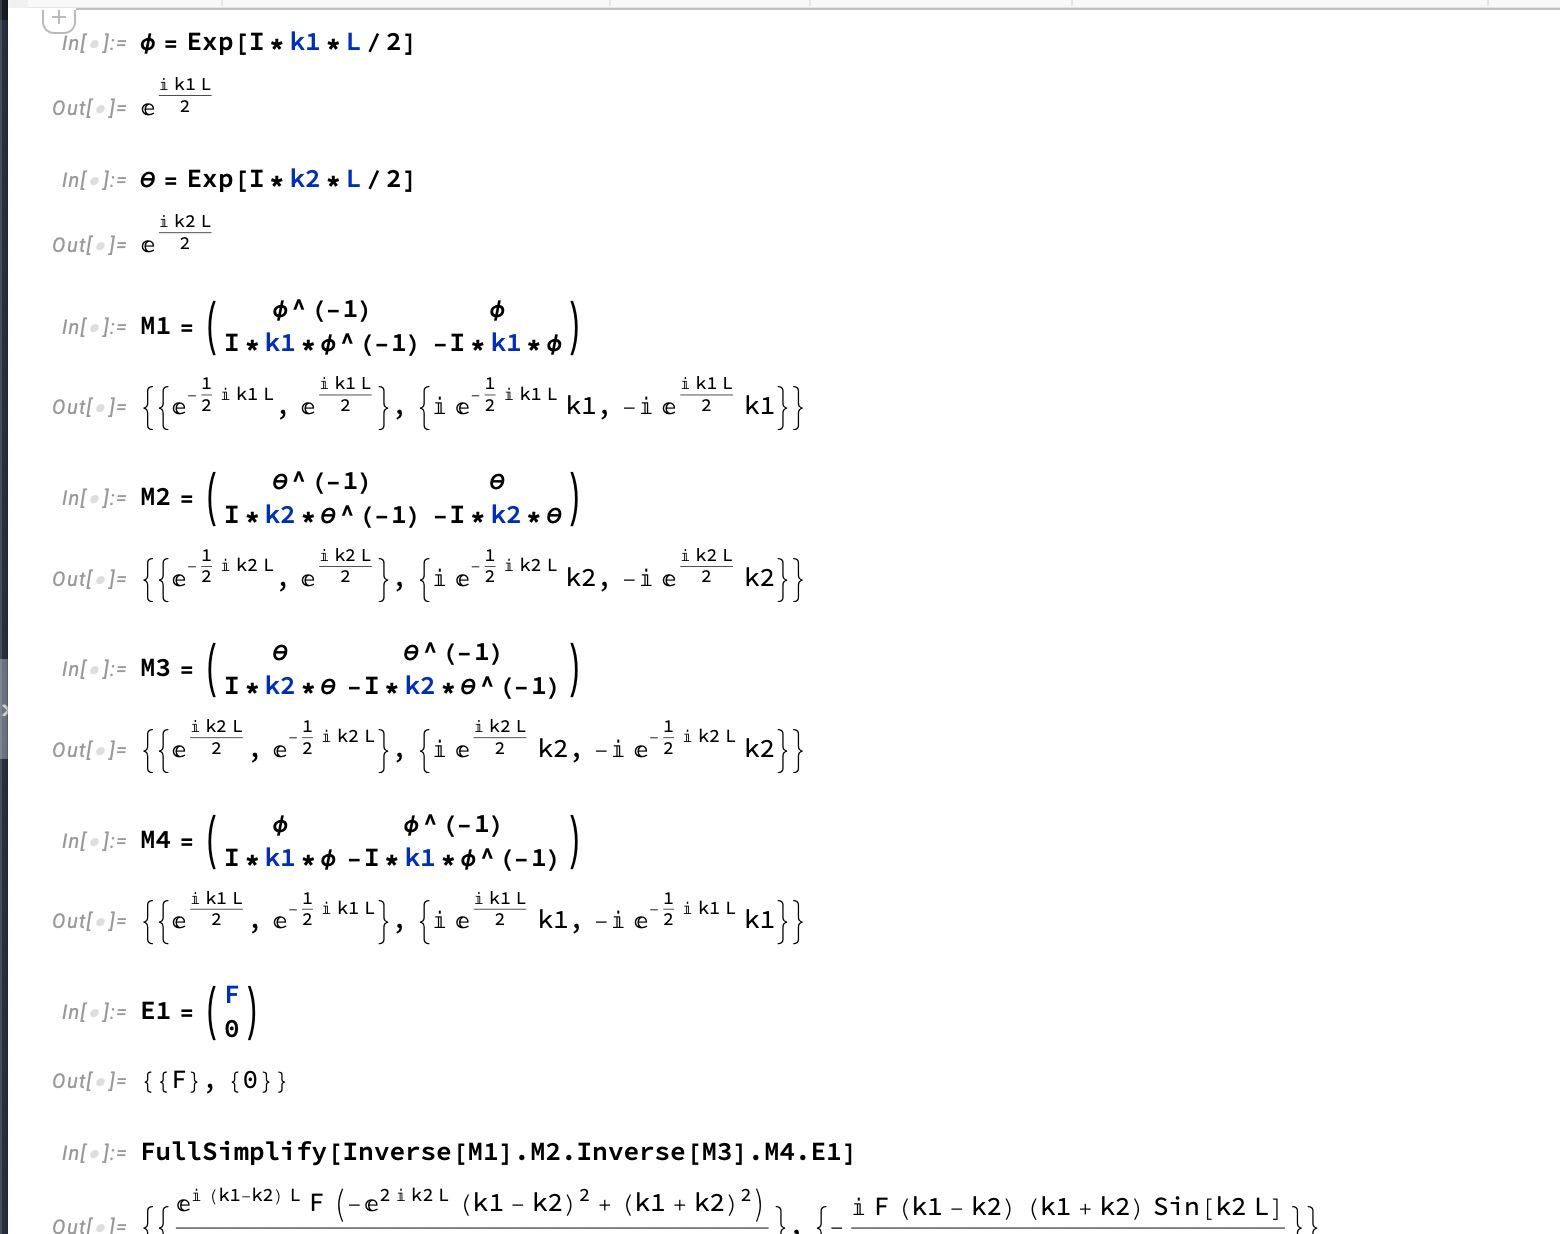
\includegraphics[width=0.8\textwidth]{./ss/9/1.png}
	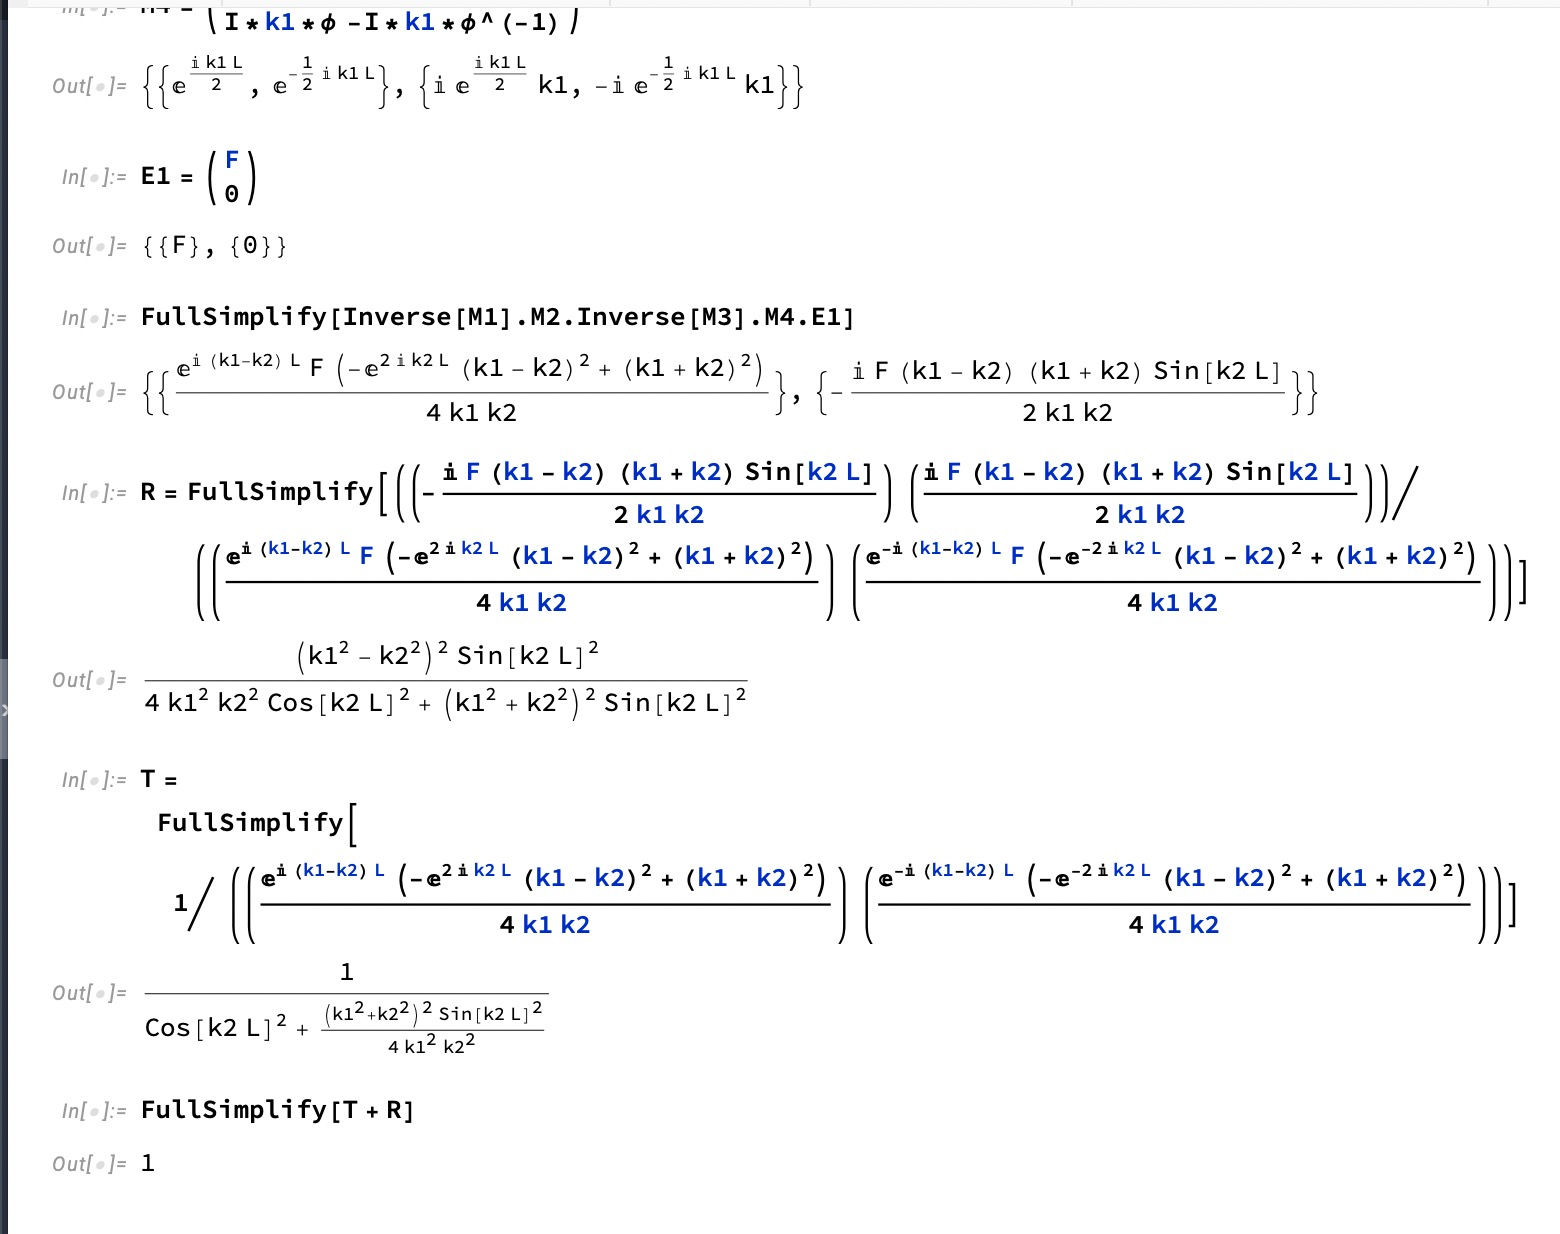
\includegraphics[width=0.8\textwidth]{./ss/9/2.png}
	\caption{./ss/9/2.png}
	\label{fig:-ss-9-2-png}
\end{figure}


Exactly putting the computation into wolfram mathematica
\begin{align*}
	\begin{bmatrix} A\\B \end{bmatrix} 
	&= 
	\begin{bmatrix} 
E
\dfrac{
e^{1+ i (k_1 - k_2) L } 
\left(
	(k_1 + k_2)^2 - (k_1 - k_2)^2 e^{2 i k_2 L}
\right)
}{4 k_1 k_2}
\\ \ \\ 	-i E 
	\dfrac{(k_1 - k_2) (k_1 + k_2) \sin (k_2 L)}{2k_1 k_2}
	\end{bmatrix} \\
\end{align*}
\begin{align*}
	\frac{B^2}{A^2} = \frac{J_B}{J_A} &= 
\frac{
	(k_1^2 - k_2^2) \sin ^2(k_2 L) 
}{4 k_1 ^2 k_2 ^2 
\cos ^2 (k_2 L) + 
(k_1 ^2 + k_2 ^2)^2 \sin ^2(k_2 L)}
	\\
	\frac{E^2}{A^2} 
	=  
	\frac{J_E}{J_A} &= 
\frac{1}{
\cos ^2 (k_2 L) 
+ 
\frac{
	(k_1 ^2 + k_2^2)^2 \sin ^2 (k_2 L)
}{4 k_1 ^2 k_2 ^2}
}
	\\
\end{align*}
\subsection*{b - i}
\begin{align*}
	T + R = \frac{J_E}{J_A} + \frac{J_B}{J_A} =
\frac{1}{
\cos ^2 (k_2 L) 
+ 
\frac{
	(k_1 ^2 + k_2^2) \sin ^2 (k_2 L)
}{4 k_1 ^2 k_2 ^2}
}+ 
\frac{
	(k_1^2 - k_2^2) \sin ^2(k_2 L) 
}{4 k_1 ^2 k_2 ^2 
\cos ^2 (k_2 L) + 
(k_1 ^2 + k_2 ^2) \sin ^2(k_2 L)} = 1
\end{align*}


\subsection*{b - ii} 
\begin{align*}
	T &= 
\frac{1}{
\cos ^2 (k_2 L) 
+ 
\frac{
	(k_1 ^2 + k_2^2)^2 \sin ^2 (k_2 L)
}{4 k_1 ^2 k_2 ^2}
}
	\\ 
	&\to 
\frac{1}{
\cos ^2 (k_1 L) 
+ 
\frac{
	(k_1 ^2 + k_1^2) ^2 \sin ^2 (k_1 L)
}{4 k_1 ^2 k_1 ^2}
} = 
\frac{1}{\cos^2 (k_1 L) + \sin ^2 (k_1 L)} = 1
\end{align*}

\subsection*{b - iii} 
\begin{align*}
T &= \frac{1}{
\cos ^2(0) + \frac{(k_1 ^2 + k_2 ^2) ^2 \sin ^2 (0 ) }{4 k_1 ^2 k_2 ^2}} = \frac{1}{1+ 0} = 1
 \\
\end{align*}


\subsection*{b - iv} 
\begin{align*}
	\cos ^2(x) \approx 
	\left(
1 - \frac{x^2}{2}  + \cdots
	\right) 
	\left(
1 - \frac{x^2}{2}  + \cdots
	\right) 
	= \left(1 - \frac{x^2}{2} - \frac{x^2}{2} + \cdots \right) =  1 - x^2 + \cdots
\end{align*}
\begin{align*}
	\lim_{k_2 \to 0} T &\approx 
\frac{1}{
1  - k_2 ^2 L ^2+ \frac{
k_1^4 k^2_2 L^2
}{4 k_1 ^2 k_2 ^2}
}
\tag{I am only keeping $k_2^2$ terms}
	\\
	&= \frac{1}{1 + \frac{k_1^2 L^2}{4}} \\
\end{align*}

\section*{Problem 05} 
Re-written form and taking a small integral from $-\varepsilon \text{ to } \varepsilon$
\begin{align*}
	\frac{\hb ^2 \lambda }{m} \delta(x) \psi(x) - E \psi(x) &= \frac{\hb^2}{2m} \frac{\mathrm{d} ^2}{\mathrm{d} x^2} \psi(x) \\ 
	\int_{- \varepsilon}^{\varepsilon} \left[
\frac{\hb^2 \lambda}{m} \delta(x- 0) \psi(x) - E \psi(x) \right] \,  \mathrm{d} x  &= 
\frac{\hb^2}{2m}
\int_{-\varepsilon}^{\varepsilon}  \frac{\mathrm{d} ^2}{\mathrm{d} x^2} \psi(x) \, \mathrm{d} x\\
\frac{\hb^2 \lambda}{m}  \psi(0)  &= 
\frac{\hb^2}{2m}
\left[
	\frac{\mathrm{d} \psi(0)_+}{\mathrm{d} x} - 
	\frac{\mathrm{d} \psi(0)_-}{\mathrm{d} x}
\right] \\
2 \lambda \psi(0)  &= 
	\frac{\mathrm{d} \psi(0)_+}{\mathrm{d} x} - 
	\frac{\mathrm{d} \psi(0)_-}{\mathrm{d} x}
\end{align*}
This gives us the discontinuity at the $x = 0$ position. 

Now using the equality of wave function $\psi(0)_< = \psi(0)_>$ on both of the sides of barrier we get
\[
A + B = C
\]
And using above discontinuity, realizing for $x\le 0$ (hence also $x = 0$ ) the wave function is given by $\psi_<(x)$, 
\[
2 \lambda \left(A + B\right) 
=
i k C - ik 
\left(
A - B
\right)
\implies 
2 \lambda C
=
i k C - ik 
\left(
A - B
\right)
\] 
Solving some algebra

\begin{minipage}{0.3\textwidth}
\begin{align*}
	2 \lambda C &= i k (C - A + B) \\ 
	2 \lambda C &= i k (A + B - A + B) \\ 
C &=  \frac{ik}{\lambda} B  \end{align*}\end{minipage}\hfill
\begin{minipage}{0.3\textwidth}
	\begin{align*}
	 \implies A+B&=C = \frac{ik}{\lambda}B \\ 
	 1 + \frac{B}{A} &= \frac{ik}{\lambda} \frac{B}{A} \\
	 1 &= \left(\frac{ik}{\lambda} - 1 \right) \frac{B}{A} \\
	 \frac{B}{A} &= \frac{1}{\dfrac{ik}{\lambda} - 1}
\end{align*}
\end{minipage}
\begin{minipage}{0.3\textwidth}
\begin{align*}
	\frac{C}{A} &= \frac{ik}{\lambda} \frac{B}{A} \\
	\frac{C}{A} &= \frac{\frac{ik}{\lambda}}{\frac{ik}{\lambda} - 1} \\
\end{align*}
\end{minipage}

To solve for following
\begin{align*}
	\frac{B}{A} &=  
	  \frac{1}{\dfrac{ik}{\lambda} - 1}\\
	\frac{C}{A} &= \frac{\frac{ik}{\lambda}}{\frac{ik}{\lambda} - 1} 
	\\
	R& =  \frac{\lambda^2}{k^2 + \lambda^2} \\ 
	T&= \frac{k^2}{\lambda^2 + k^2} \\
	R + T &= 1 
\end{align*}
\end{document}
